\input{../../style/preamble} 
\input{../../latex-math/basic-math}
\input{../../latex-math/basic-ml}
\input{../../latex-math/ml-bagging.tex}
\input{../../latex-math/ml-boosting.tex}
\input{../../latex-math/ml-trees.tex}

\newcommand{\titlefigure}{figure_man/componentwise-gb.png}
\newcommand{\learninggoals}{
  \item Learn the concept of componentwise boosting and its relation to GLM
  \item Understand the built-in feature selection process
  \item Understand the problem of fair base learner selection
}

\title{Introduction to Machine Learning}
\date{}

\begin{document}

\lecturechapter{Componentwise Gradient Boosting}
\lecture{Introduction to Machine Learning}

% ------------------------------------------------------------------------------

\begin{vbframe}{Componentwise gradient boosting}

Gradient boosting, especially when using trees, has strong predictive
performance but is difficult to interpret unless the base learners are stumps.

\lz

The aim of componentwise gradient boosting is to find a model that:

\begin{itemize}
  \item
    has strong predictive performance,

  \item
    has components that are still interpretable,

  \item
    does automatic selection of components,

  \item
    is sparser than a model fitted with maximum-likelihood estimation.
\end{itemize}

\lz

This is achieved by using \enquote{nice} base learners which yield familiar 
statistical models
in the end.

\lz

Because of this, componentwise gradient boosting is also often referred to as \textbf{model-based boosting}.

\end{vbframe}

% ------------------------------------------------------------------------------

\begin{vbframe}{Base learners}

In classical gradient boosting only one kind of base learner $\mathcal{B}$ is used, e.g., 
regression trees.

\lz

For componentwise gradient boosting we generalize this to multiple base learner sets $\{ \mathcal{B}_1, ... \mathcal{B}_J \}$.
% $$
%   % b_j^{[m]}(\xv,\pmb\theta^{[m]}) \quad j = 1,\dots, J\,,
%   \{ \bmm_j(\xv, \thetam): j = 1, 2, \dots, J \},
% $$
% 
 where $j$ indexes the type of base learner.
% 
% \lz

Again, in each iteration, only the best base learner 
$\bmm_{\hat{j}}(\xv, \thetam)$ is selected and updated.

\end{vbframe}
% ------------------------------------------------------------------------------

\begin{vbframe}{Componentwise boosting algorithm}


\begin{algorithm}[H]
  \begin{footnotesize}
  \begin{center}
  \caption{Componentwise Gradient Boosting.}
    \begin{algorithmic}[1]
      \State Initialize $f^{[0]}(\xv) = \argmin_{\theta} \sum  \limits_{i=1}^n L(\yi, \theta)$
      \For{$m = 1 \to M$}
        \State For all $i$: $\rmi = -\left[\fp{L(\yi, f(\xi))}{f(\xi)}\right]_{f=\fmd}$
        \For {$j= 1\to J$}
          \State Fit regression base learner $b_j \in \mathcal{B}_j$ to the pseudo-residuals $\rmi$:
          \State $\thetamh_j = \argmin_{\pmb\theta_j} \sum  \limits_{i=1}^n 
          (\rmi - b_j(\xi, \pmb\theta_j))^2$
        \EndFor
        \State $\hat{j} = \argmin_{j} \sum  \limits_{i=1}^n (\rmi - \hat{b}_j(\xi, \thetamh_j))^2$
        \State Update $\fm(\xv) = \fmd(\xv) + \beta \hat{b}_{\hat{j}}(\xv, \thetamh_{\hat{j}})$
      \EndFor
      \State Output $\fh(\xv) = f^{[M]}(\xv)$
    \end{algorithmic}
    \end{center}
    \end{footnotesize}
\end{algorithm}


\end{vbframe}
% ------------------------------------------------------------------------------
\begin{vbframe}{Additive model structure}
\begin{footnotesize}
We restrict these base learners to additive models, i.e., having a base learner $ b_j(\xv, \thetab^{[1]})$ and another base learner $b_j$ of the same type but with a different parameter vector $\thetab^{[2]}$, then it is possible to combine them to a new base learner of the same type:

$$
 b_j(\xv, \thetab^{[1]}) + b_j(\xv, \thetab^{[2]}) = 
 b_j(\xv, \thetab^{[1]} + \thetab^{[2]}).
$$
\vspace*{0.1cm}

Thus, if $\{ b_j(\xv, \thetab^{[1]}), b_j(\xv, \thetab^{[2]}) \} \in \mathcal{B}_j$, then $b_j(\xv, \thetab^{[1]} + \thetab^{[2]}) \in \mathcal{B}_j$.
\lz

Often base learners are not defined on the entire feature vector $\xv$ but on 
a single feature $x_j$:

$$
  b_j(x_j, \theta) \quad \text{for } j = 1, 2, \dots, p.
$$

This directly incorporates a variable selection mechanism into the fitting 
process, since in each iteration only the best base learner is selected in 
combination with the associated feature, and each base learner can be 
(substantially) more complex than a stump (e.g., univariate linear effects or 
splines).
\end{footnotesize}
\end{vbframe}



% ------------------------------------------------------------------------------

\begin{vbframe}{relation to glm}

In the simplest case we use linear models (without intercept) on single features 
as base learners:

$$
  b_j(x_j,\theta) = \theta x_j  \quad \text{for } j = 1, 2, \dots, p \quad
  \text{and with } b_j \in \mathcal{B}_j = \{\theta x_j  ~\rvert~ \theta \in 
  \mathbb{R} \}.
$$


This definition will result in an ordinary \textbf{linear regression} model 
(note that linear base learners without intercept only make sense for covariates 
that have been centered before).

% .\footnote{Note: a linear model base learner without intercept only makes sense if the covariates are centered (see \texttt{mboost} tutorial, page7)}


\begin{itemize}
  \item If we let the boosting algorithm converge, i.e., let it run for a really 
  long time, the parameters estimated by the boosting model will converge to the 
  \textbf{same solution} as the ML estimate.
  \item This means that, by specifying a loss function according to the negative 
  likelihood of a distribution from an exponential family and defining a link 
  function accordingly, this kind of boosting is equivalent to a (regularized)
  \textbf{generalized linear model (GLM)}.
\end{itemize}

\framebreak

% ------------------------------------------------------------------------------

But: We do not \emph{need} an exponential family and thus are able to fit models 
to all kinds of other distributions and losses, as long as we can calculate (or 
approximate) a derivative of the loss. 
% Note, however, that this does not imply that the algorithm does something 
% meaningful (e.g., non-convex loss functions would still require some 
% additional effort).

\lz

Usually we do not let the boosting model converge fully, but \textbf{stop 
early} for the sake of regularization and feature selection.

\lz

Even though the resulting model looks like a GLM, we do not have valid standard 
errors for our coefficients,
so cannot provide confidence or prediction intervals or perform tests etc.
$\rightarrow$ post-selection inference.

\end{vbframe}

% ------------------------------------------------------------------------------

\begin{vbframe}{example: feature selection for titanic}

\small
Consider the \texttt{titanic} data, for which we fit a componentwise gradient 
boosting model with linear base learners, using the R package \texttt{compboost} 
with $M = 200$, to predict passengers' survival.
We can visualize the updates of the $\theta_j$ over time to see which base 
learner was selected when.

\vfill

\begin{center}
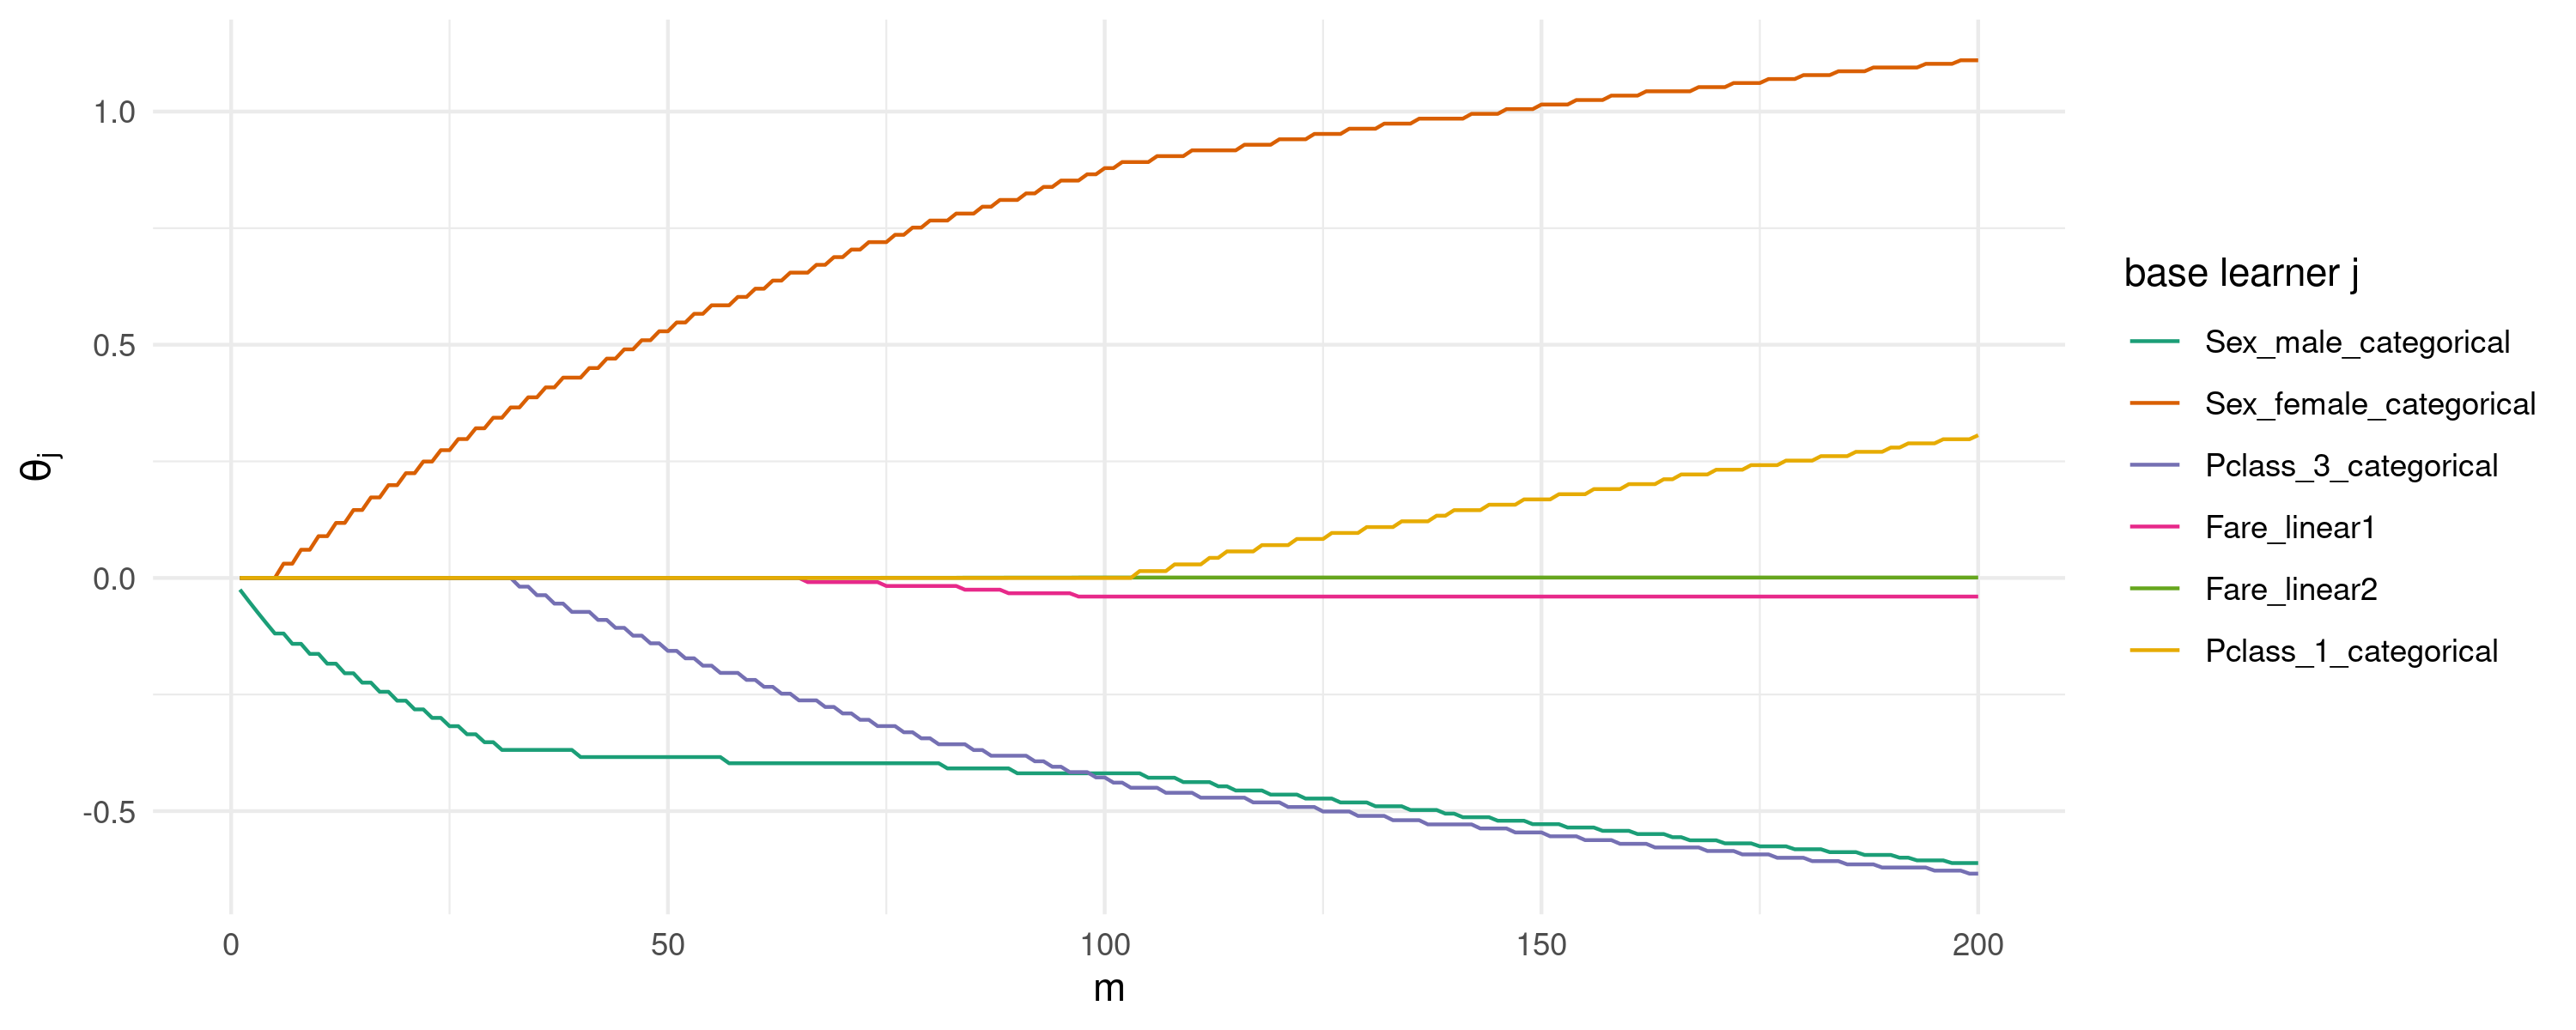
\includegraphics[width = \textwidth]{figure/compboost-illustration-1.png}
% \includegraphics[width=0.9\textwidth]{figure_man/componentwise-gb.png}
\end{center}

\vfill

\small
New variables are added cautiously, yielding a rather parsimonious model.
Being male and/or traveling in the bottom class clearly bodes ill for surival.

\framebreak

% ------------------------------------------------------------------------------



% ------------------------------------------------------------------------------

The number of features effectively included in the final model depends on the 
number of total iterations $M$.

\vfill

$\rightarrow$ A sparse logistic regression is fitted.

\vfill

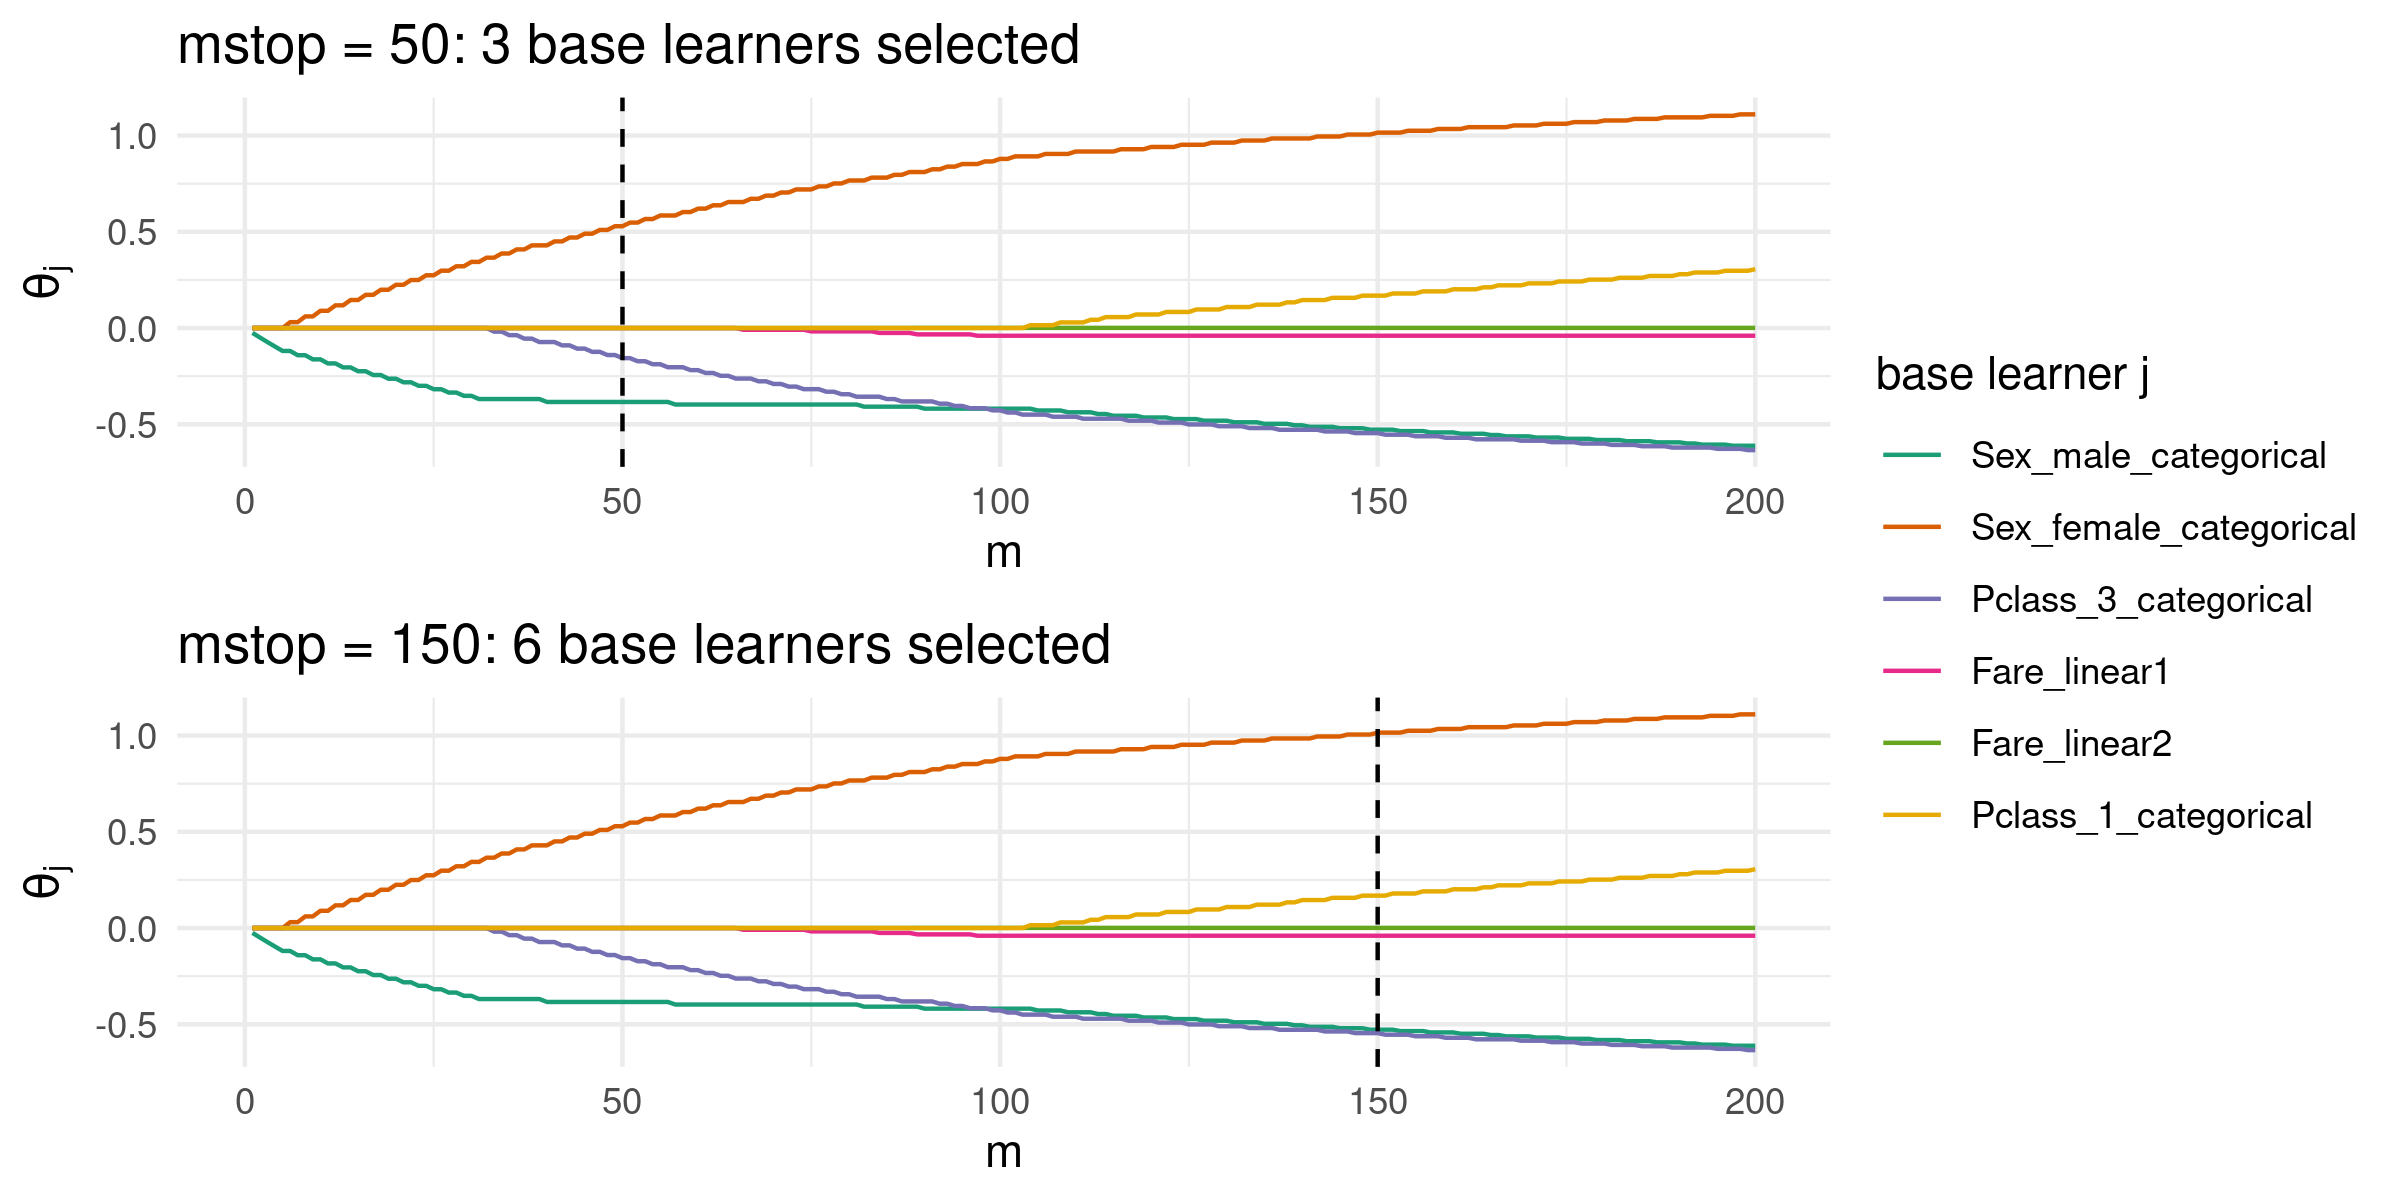
\includegraphics[width = \textwidth]{figure/compboost-illustration-2.png}

\end{vbframe}

% ------------------------------------------------------------------------------

\begin{vbframe}{Nonlinear base learners}

Nonlinear base learners like $P$- or $B$-splines make the model equivalent to a
\textbf{generalized additive model (GAM)}, as long as the base learners keep 
their additive structure (which is the case for splines).
\vspace{0.5cm}

\vfill

\begin{center}
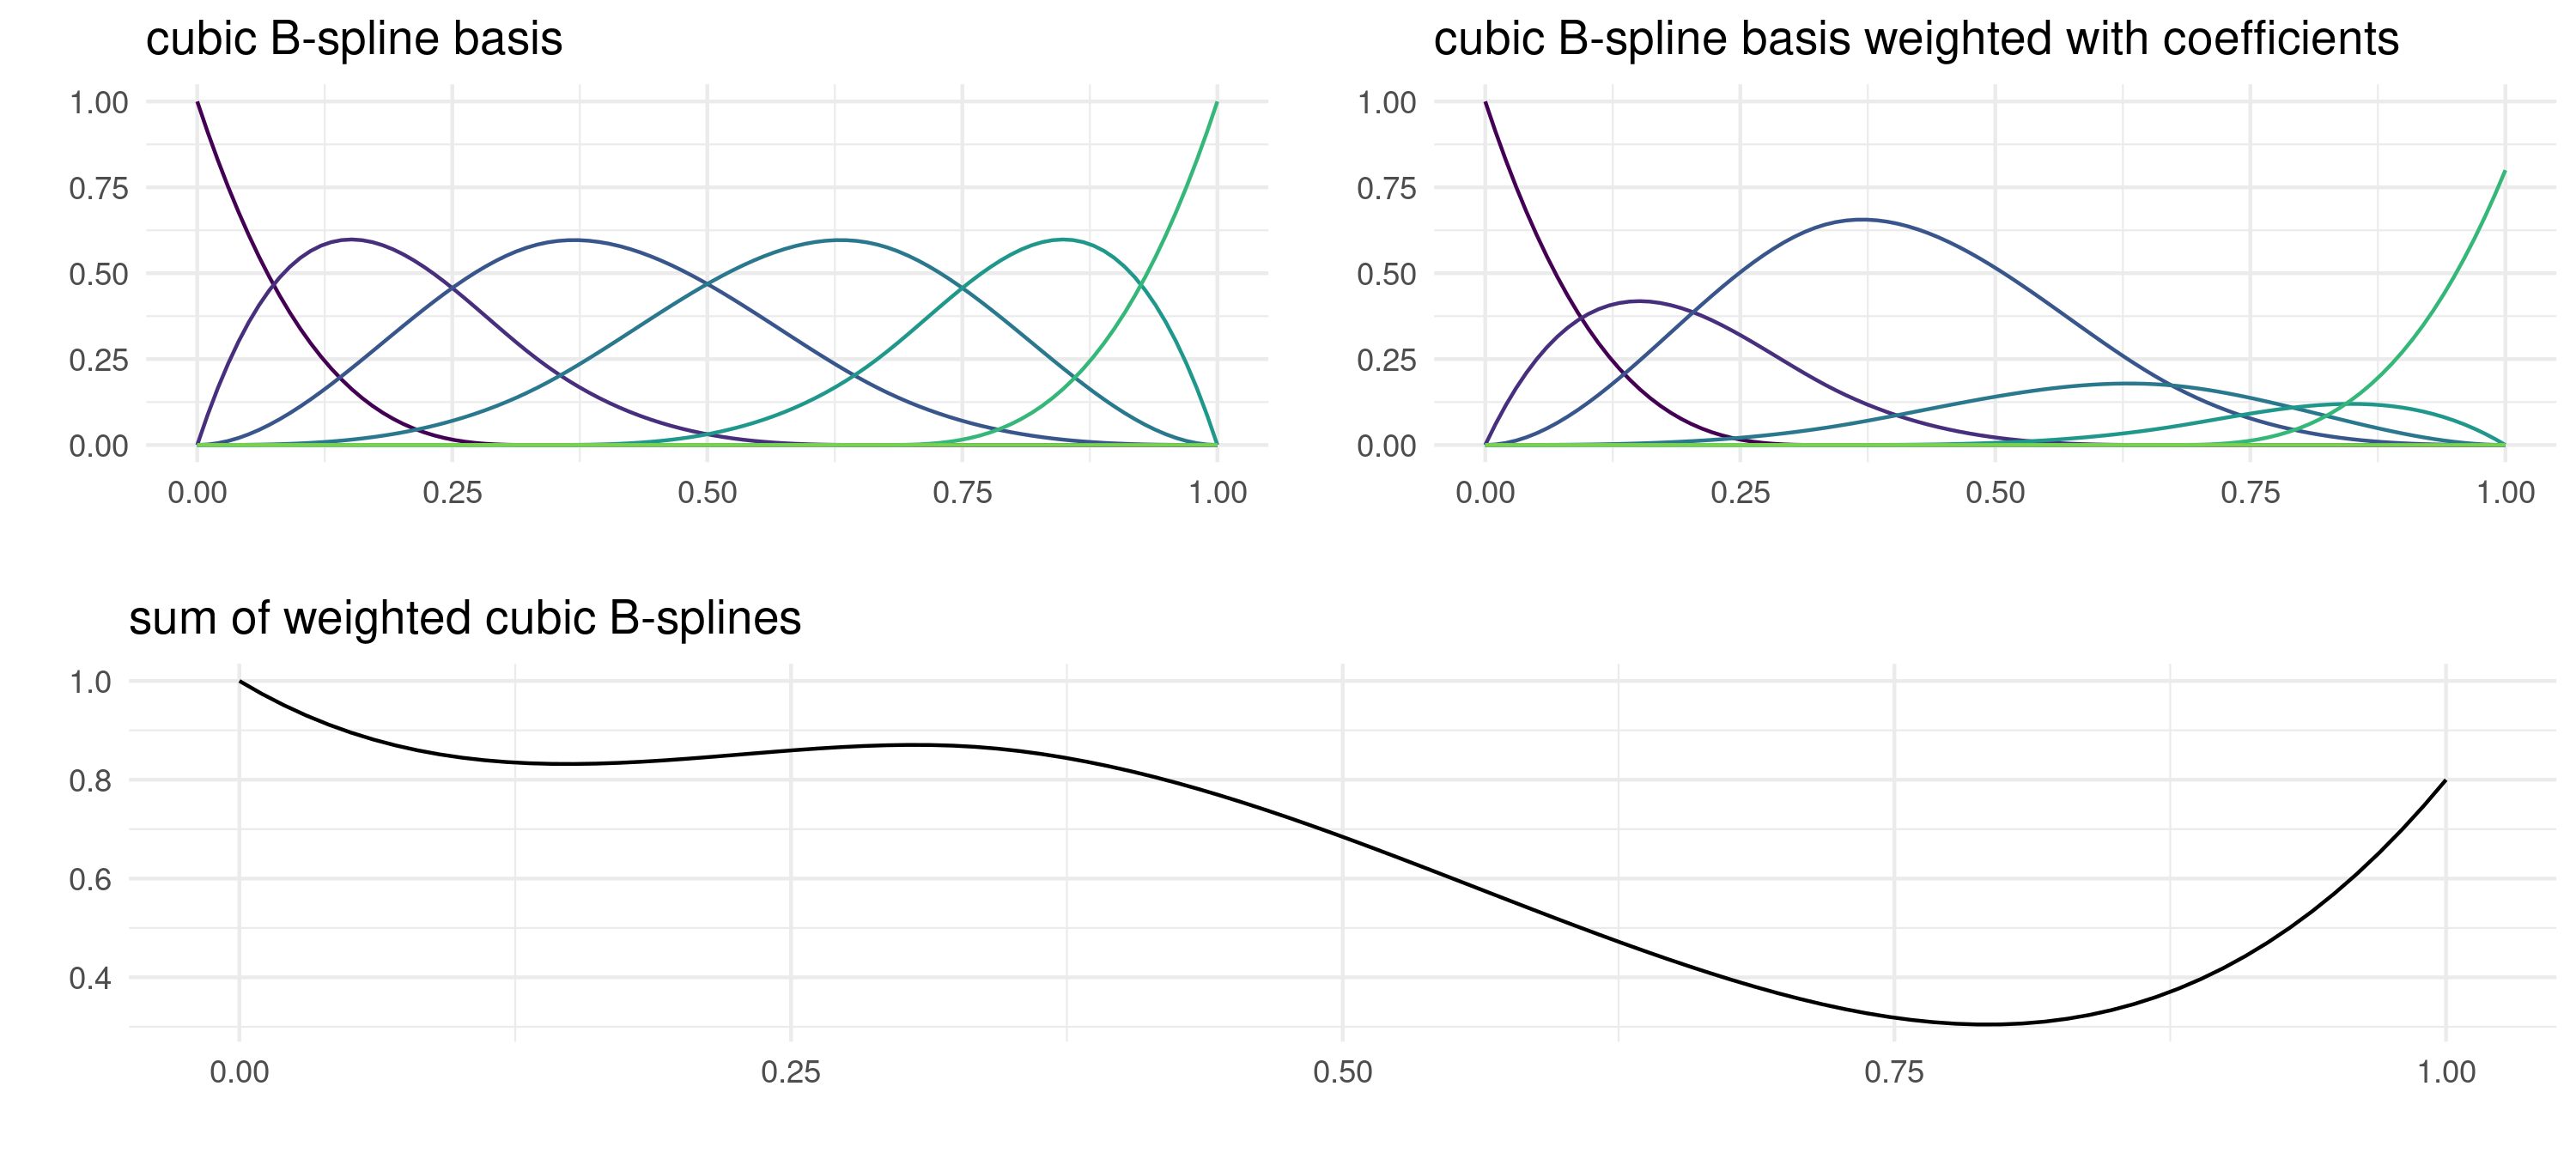
\includegraphics[width=1\textwidth]{figure/bspline-basis.png}
\end{center}

% \vfill
% 
% \begin{center}
% \includegraphics[width=1\textwidth]{figure_man/NBL02.png}
% \end{center}

\framebreak

% ------------------------------------------------------------------------------

Even when allowing for more complexity we typically want to keep solutions as 
simple as possible.

\lz

Kneib~et~al. (2009) proposed a decomposition of each base learner into a 
constant, a linear and a nonlinear part. 
The boosting algorithm will automatically decide which feature to include -- 
linear, nonlinear, or none at all:

\vspace{-0.5cm}

\begin{align*}
b_j(x_j, \thetam) & = b_{j, \text{const}}(x_j, \thetam) + b_{j, \text{lin}}
(x_j, \thetam) + b_{j, \text{nonlin}}(x_j, \thetam)\\
 & = \theta^{[m]}_\text{const} + x_j \cdot \theta^{[m]}_{j, \text{lin}} + 
 s_j(x_j, \thetam_{j,\text{nonlin}}),
\end{align*}

\small
where
\begin{itemize}
  \small
  \item $\theta_\text{const}$ is a constant term over all base learners,
  \item $x_j \cdot \theta^{[m]}_{j, \text{lin}}$ is a feature-specific linear 
  base learner, and
  \item $s_j(x_j, \thetam_{j,\text{nonlin}})$ is a (centered) nonlinear base 
  learner capturing deviation from the linear effect.
\end{itemize}

\end{vbframe}

% ------------------------------------------------------------------------------

\begin{vbframe}{titanic example: continued}

\begin{itemize}
  \small
  \item This time we offer our model both 
  linear and nonlinear ($B$-spline) base learners for the numeric features.
  \item By iteration 200, the model has selected 6 out of 16 features, 3 of 
  which are categorical (concerning sex and passenger class).
  \item For the 3 numeric ones, the model always picks the nonlinear option. 
  We can trace how they evolve over the iterations:
\end{itemize}

\vfill

\begin{center}
% \includegraphics[width=0.6\textwidth]{figure_man/spam-example.png}
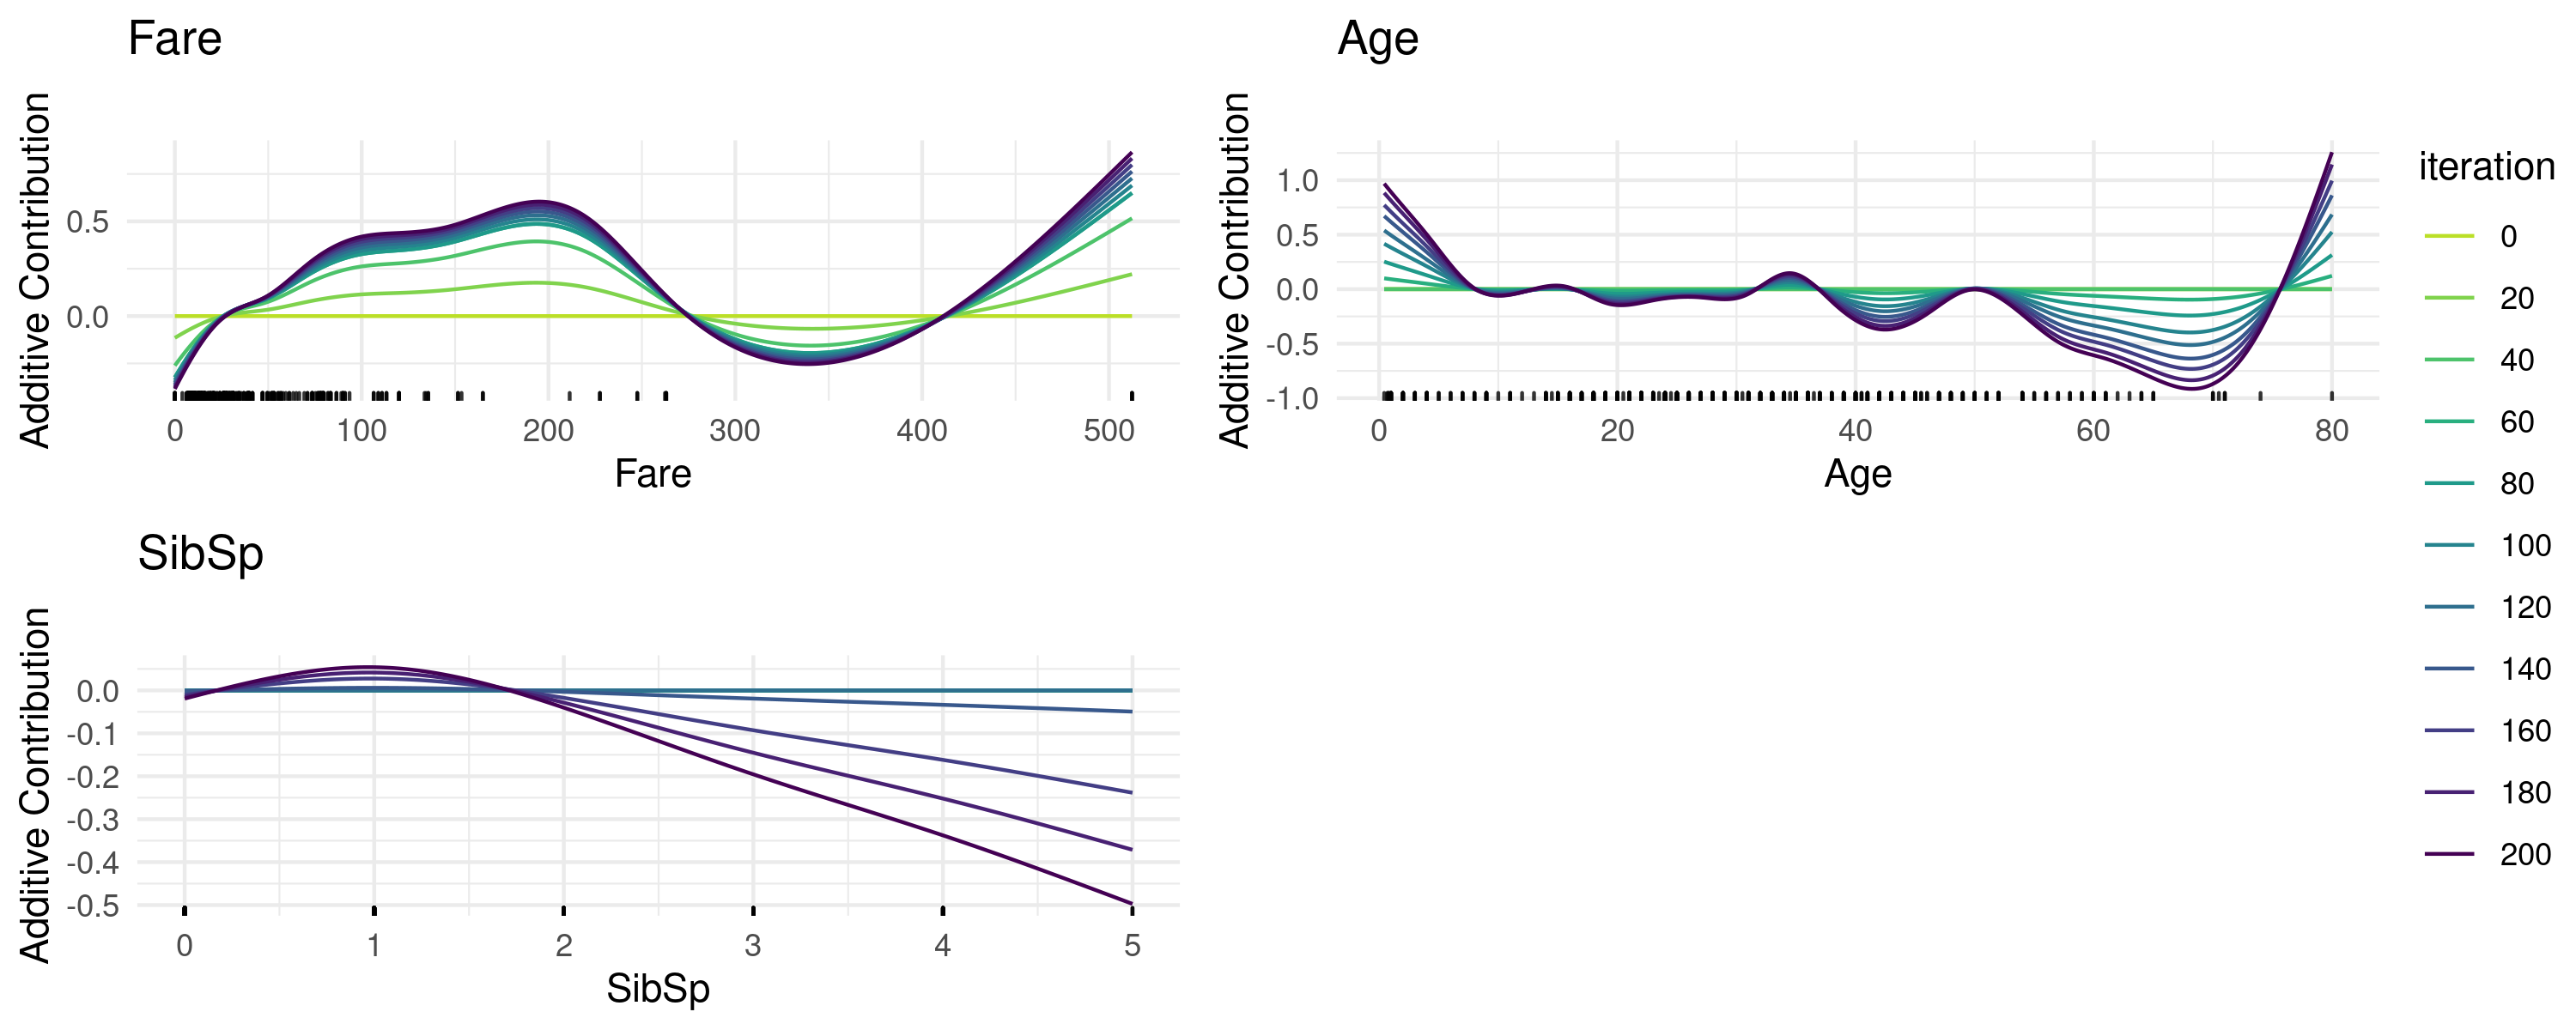
\includegraphics[width = \textwidth]{figure/compboost-illustration-3.png}
\end{center}

% Unfortunately it's rather ugly to write down the decomposition

% <<spam-formula, eval = FALSE, echo = TRUE>>=
% formula <-
%   spam ~ bols(word_freq_make) + bbs(word_freq_make, df = 2, center = TRUE) +
%     bols(word_freq_address) + bbs(word_freq_address, df = 2, center = TRUE) +
%     bols(word_freq_all) + bbs(word_freq_all, df = 2, center = TRUE) +
% #  ...
% mboost(formula, data = spam, family = Binomial(), control = boost_control(mstop = 100))
% @

\end{vbframe}

% ------------------------------------------------------------------------------

\begin{vbframe}{Fair Base Learner Selection}

\begin{itemize}

  \item
    Using splines and linear base learners in componentwise boosting will favor 
    the more complex spline base learner over the linear base learner.

  \item
    This makes it harder to achieve the desired behavior of the base learner 
    decomposition as explained previously.

  \item
    To conduct a fair base learner selection we set the degrees of freedom of all base learners equal.

  \item
    The idea is to set the regularization/penalty term of a single learner in a manner that their complexity is treated equally.

\end{itemize}

\framebreak

% ------------------------------------------------------------------------------

Especially for linear models and GAMs it is possible to transform the degrees of freedom into a corresponding penalty term.
\begin{itemize}

  \item
    Parameters of the base learners are estimated via:
    $$
    \thetam_j = \left(\mathbf{Z}_j^T \mathbf{Z}_j + \lambda_j \mathbf{K}_j
    \right)^{-1}\mathbf{Z}_j^T \rmm\,,
    $$
    with $\mathbf{Z}_j$ the design matrix of the $j$-th base learner, 
    $\lambda_j$ the penalty term, and $\mathbf{K}_j$ the penalty matrix.

  \item
    Having that kind of model, we use the hat matrix 
    $\mathbf{S}_j = \mathbf{Z}_j\left(\mathbf{Z}_j^T \mathbf{Z}_j + 
    \lambda_j \mathbf{K}_j\right)^{-1}\mathbf{Z}_j^T$ to define the degrees of 
    freedom:
    $$
    \operatorname{df}(\lambda_j) = \trace\left(2\mathbf{S}_j - \mathbf{S}_j^T
    \mathbf{S}_j\right).
    $$
    \textbf{Note:} With $\lambda_j = 0$, $\mathbf{S}_j$ is the projection matrix 
    into the target space with 
    $\trace(\mathbf{S}_j) = \operatorname{rank}(\Xmat)$, which corresponds to 
    the number of parameters in the model.

\end{itemize}

\framebreak

% ------------------------------------------------------------------------------

It is possible to calculate $\lambda_j$ by applying the Demmler-Reinsch 
orthogonalization (see 
\href{https://www.tandfonline.com/doi/abs/10.1198/jcgs.2011.09220}
{Hofer et al. (2011)}).

% (see Hofer et. al. (2011).\textit{\enquote{A framework for unbiased model selection based on boosting.}}). 

Consider the following example of a GAM using splines with 24 parameters:

\begin{itemize}

  \item
    Setting $\operatorname{df} = 24$ gives $B$-splines with $\lambda_j = 0$.

  \item
    Setting $\operatorname{df} = 4$ gives $P$-splines with $\lambda_j = 418$.

  \item
    Setting $\operatorname{df} = 2$ gives $P$-splines with $\lambda_j = 42751174892$.

\end{itemize}

\begin{center}
\includegraphics[width=0.7\textwidth]{figure_man/df_to_lambda.pdf}
\end{center}

\end{vbframe}

\begin{vbframe}{Available base learners}

There is a large amount of possible base learners, e.g.:

\begin{itemize}
  \item Linear effects and interactions (with or without intercept)
  \item Uni- or multivariate splines and tensor product splines
  \item Trees
  \item Random effects and Markov random fields
  \item Effects of functional covariates
  \item ...
\end{itemize}

\lz

In combination with the flexible choice of loss functions, this allows boosting to fit  a huge number of different statistical models with the same algorithm. Recent extensions include GAMLSS-models, where multiple additive predictors are boosted to model different distribution parameters (e.g., conditional mean and variance for a Gaussian model).

\end{vbframe}
% ------------------------------------------------------------------------------
\begin{vbframe}{Partial Dependence Plots (PDP)}

If we use single features in base learners, we think of each base learner as a wrapper around a feature which represents the effect of that feature on the target variable. Base learners can be selected more than once (with varying parameter estimates), signaling that this feature is more important.\\
E.g. let $j \in \{ 1,2,3 \}$, the first three iterations might look as follows
\begin{align*}
m = 1: \quad & \hat{f}^{[1]}(\xv) = \hat{f}^{[0]} + \beta \textcolor{blue}{\hat{b}_2(x_2, \hat{\theta}^{[1]})}\\
m = 2: \quad & \hat{f}^{[2]}(\xv) = \hat{f}^{[1]} + \beta  \textcolor{orange}{\hat{b}_3(x_3, \hat{\theta}^{[2]})}\\
m = 3: \quad & \hat{f}^{[3]}(\xv) = \hat{f}^{[2]} + \beta \textcolor{blue}{\hat{b}_2(x_2, \hat{\theta}^{[3]})}
\end{align*}

Due to linearity, $\hat{b}_2$ base learners can be aggregated:
$$
\hat{f}^{[3]}(\xv) = \hat{f}^{[0]} + \beta (\textcolor{blue}{\hat{b}_2(x_2, \hat{\theta}^{[1]} + \hat{\theta}^{[3]})} + \textcolor{orange}{\hat{b}_3(x_3, \hat{\theta}^{[2]})})
$$

Which is equivalent to:
$\hat{f}^{[3]}(\xv) = \hat{f}_0 + \textcolor{blue}{\hat{f}_2(x_2)} + \textcolor{orange}{\hat{f}_3(x_3)}$.\\
Hence, $\hat{f}$ can be decomposed into the marginal feature effects (PDPs).



\end{vbframe}




\begin{vbframe}{Feature importance}
\begin{itemize}
  \item We can further exploit the additive structure of the boosted ensemble to 
  compute measures of \textbf{variable importance}.
  \item To this end, we simply sum for each feature $x_j$ the improvements in 
  empirical risk achieved over all iterations until 
  $1 < m_{\text{stop}} \leq M$:
  % \begin{align*}
    $$VI_j = \sum_{m = 1}^{m_{\text{stop}}} \left( \riske \left(
    \fmd(\xv) \right) - \riske \left(\fm(\xv) 
    \right) \right) \cdot \I_{[j \in sel(m)]},$$
  % \end{align*}
  where $sel(m)$ denotes the index set of features selected in the $m$-th 
  iteration.
\end{itemize}

\end{vbframe}

\begin{vbframe}{Available base learners}

There is a large amount of possible base learners, e.g.:

\begin{itemize}
  \item Linear effects and interactions (with or without intercept)
  \item Uni- or multivariate splines and tensor product splines
  \item Trees
  \item Random effects and Markov random fields
  \item Effects of functional covariates
  \item ...
\end{itemize}

\lz

In combination with the flexible choice of loss functions, this allows boosting to fit  a huge number of different statistical models with the same algorithm. Recent extensions include GAMLSS-models, where multiple additive predictors are boosted to model different distribution parameters (e.g., conditional mean and variance for a Gaussian model).

\end{vbframe}

% ------------------------------------------------------------------------------

% \begin{vbframe}{RF vs AdaBoost vs GBM vs Blackboost}

% Again the Spirals data from mlbench. Blackboost: mboost with regression trees as base learners
% \end{vbframe}

\begin{vbframe}{Take-home message}

\begin{itemize}
  \item Componentwise gradient boosting is the statistical re-interpretation of 
  gradient boosting.
  \item We can fit a large number of statistical models, even in high dimensions 
  ($p \gg n$).
  \item A drawback compared to statistical models is that we do not get valid 
  inference for coefficients $\rightarrow$ post-selection inference.
  % This can be (partially) solved by bootstrap inference or related methods.
  \item In most cases, gradient boosting with tree will dominate componentwise 
  boosting in terms of performance due to its inherent ability to include 
  higher-order interaction terms.
  % In most cases, componentwise gradient boosting will have worse 
  % predictive performance than gradient boosting with trees. This is often 
  % because additive base learner motivated by regression models (LM, GLM, GAM) 
  % usually do not include higher-order interaction terms.
\end{itemize}

\end{vbframe}

% ------------------------------------------------------------------------------

\endlecture
\end{document}
